% mainfile: ../../../../master.tex
\subsection{Explore Migration of Zicheng's Works to AOSP14}
\label{task:20240116_aosp}

\subsubsection{Clone AOSP14}

Tried cloning AOSP 14 into new directory:
\begin{lstlisting}[language=bash]
mkdir aosp14 && cd aosp14
repo init -u https://android.googlesource.com/platform/manifest -b android-14.0.0.r_21
\end{lstlisting}
But faced this error:
\begin{lstlisting}
manifests:
fatal: couldn't find remote ref refs/heads/android-14.0.0.r_21
manifests: sleeping 4.0 seconds before retrying
fatal: cannot obtain manifest https://android.googlesource.com/platform/manifest
================================================================================
Repo command failed: UpdateManifestError
    Unable to sync manifest default.xml
\end{lstlisting}

Checking the available branches with:
\begin{lstlisting}[language=bash]
git ls-remote -h https://android.googlesource.com/platform/manifest.git
\end{lstlisting}
And the result is:
\begin{lstlisting}
...
06e1764f504727281253313fbf6c227cebd65e4c	refs/heads/android-13.0.0_r79
2f7b75202188e6deee159b2dea97719a51f63c2f	refs/heads/android-13.0.0_r8
4ca496b8eaa717f861e193233cd3917d9fbbb5a7	refs/heads/android-13.0.0_r80
259db423b147ea6f75b25a87a47190a17b1fda10	refs/heads/android-13.0.0_r81
ed487956fff8d6b616d99ace142203d6b89aa877	refs/heads/android-13.0.0_r82
f5d5c1675fabbca4cebc0d1b618ff6f7b6f14025	refs/heads/android-13.0.0_r83
0bac787fd054b65de0e755dd8f32b1f07cc0b485	refs/heads/android-13.0.0_r9
e3f9241982f55ef4cec97df0c55e9b87d37a5656	refs/heads/android-14.0.0_r1
32f134303b62e8815287a61ad285cc0171fb3091	refs/heads/android-14.0.0_r10
29fddb193223ac701779eb45a926b21e9e6c9585	refs/heads/android-14.0.0_r11
1ea2801d54e826ea03e3a6c33e09c2c36da4df41	refs/heads/android-14.0.0_r12
ab70a6753ba6dfa223eec03762de67a3e001111f	refs/heads/android-14.0.0_r13
d774d22bad0a0dcc3494566b52f48b40afb2c0dd	refs/heads/android-14.0.0_r14
323da1dc43d2c9ace9f97ddf5744fdbeb5c0d4e7	refs/heads/android-14.0.0_r15
e43bd2ae656e593e68015f922b7f5b1af335bf0c	refs/heads/android-14.0.0_r16
d091bf89b3c2e459dc46fe4238695205990228a8	refs/heads/android-14.0.0_r17
dcd243f609d59f6d919660898949775d0976ed0b	refs/heads/android-14.0.0_r18
bd6b6c3427247e3cdf23c4daafdd4e050488aadb	refs/heads/android-14.0.0_r19
cae010b8c39e45a9fc675fce989a284c5e39ebed	refs/heads/android-14.0.0_r2
d25293c4ced217d523f7773a3426fee6e8c5160c	refs/heads/android-14.0.0_r20
ce85fafc1db1bafbe98e326a9ac1fde211f0495d	refs/heads/android-14.0.0_r21
...
\end{lstlisting}

The branch of our current AOSP 13 according to \path{.repo/manifests/default.xml} is:
\begin{lstlisting}[language=xml]
<?xml version="1.0" encoding="UTF-8"?>
    <manifest>
    
      <remote  name="aosp"
               fetch=".."
               review="https://android-review.googlesource.com/" />
      <default revision="refs/tags/android-13.0.0_r11"
               remote="aosp"
               sync-j="4" />
\end{lstlisting}

Instead of switching branch to a totally different android version, try switching to another branch of 13:
\begin{lstlisting}[language=bash]
cd aosp13
repo init -u https://android.googlesource.com/platform/manifest -b android-13.0.0.r_83
\end{lstlisting}
Also fail! STUPID ERROR! should \texttt{\_r83}, NOT \texttt{.r\_83}! NOW FIXED! Cloning into new directory now.



% \begin{itemize}
% \item \textbf{Domain.} The context of the process that is acting upon something.
% \item \textbf{Type.} The context of the resource on which the process is acting.
% \item \textbf{Class.} The object class of the resource (e.g. \textit{file} or \textit{socket}).
% \item \textbf{Permissions.} The permissions that are allowed given the \textit{domain}, \textit{type} and \textit{class}.
% \end{itemize}

% SELinux rule syntax:
% \begin{lstlisting}
% allow <domain> <type>:<class> { <permissions> };
% \end{lstlisting}

% \subsubsection{Decoding Permission Denial Message}

% Message:
% \begin{lstlisting}
% type=AVC msg=audit(1363289005.532:184): avc:  denied  { read } for  pid=29199 comm="Trace" 
% name="online" dev="sysfs" ino=30 scontext=staff_u:staff_r:googletalk_plugin_t 
% tcontext=system_u:object_r:sysfs_t tclass=file
% \end{lstlisting}

% \begin{longtable}{p{.15\linewidth}p{.15\linewidth}p{.65\linewidth}} 
% \toprule
% Log part & Name & Description \\
% \midrule
% \endhead

% \texttt{type=AVC}
% &Log type
% &Only in the \texttt{audit.log} file; it informs the user what kind of audit log type this is. 
% \\

% \texttt{msg=audit(1363289005.532:184)}
% &Timestamp
% &Timestamp in seconds since epoch, meaning the number of seconds since January 1st, 1970. You can convert this to a more human readable format using date -d @ followed by the number, like so: \texttt{date -d @1363292159.532}.
% \\

% \texttt{avc:}
% &Log type (again)
% &
% \\

% \texttt{ino=30}
% &inode number
% &The inode number of the target file. In this case, since we know it is on the \texttt{sysfs} file system, we can look for this file using: \texttt{find /sys -xdev -inum 30}
% \\

% \texttt{scontent=staff\_u:staff\_r:googletalk\_plugin\_t}
% &Source context
% &The security context of the process (the domain)
% \\

% \texttt{tcontext=system\_u:object\_r:sysfs\_t}
% &Target context
% &The security context of the target resource (in this case the file)
% \\

% \texttt{tclass=file}
% &Target class
% &The class of the target.
% \\

% \midrule
% \caption{Permission Denied Syntax} 
% \label{tab:permissiondeniedsyntax}
% \end{longtable}


% \subsubsection{SELinux Architecture}

% SELinux consists of four main components: object managers (OM), access vector cache (AVC), security server, and security policy as show below:
% \begin{figure}[H]
%     \centering
%     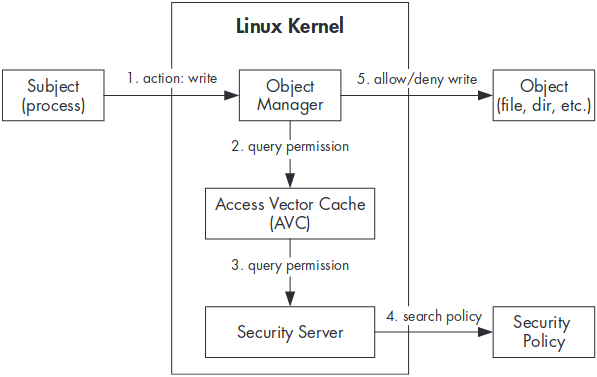
\includegraphics[width=.85\linewidth]{entries/2023/12/10/selinux.png}
%     \caption{SELinux Components}
%     \label{fig:selinux}
% \end{figure}
